%---------------------------------------------------------------------------
%	PACKAGES AND OTHER DOCUMENT CONFIGURATIONS
%---------------------------------------------------------------------------
\documentclass[final]{beamer}
\usepackage{gensymb}
\usepackage{textcomp}
\usepackage{overpic}
\usepackage{bm}
\usepackage[scale=1]{beamerposter} % Use the beamerposter package for laying out the poster
\usetheme{confposter} % Use the confposter theme supplied with this template
\setbeamercolor{block title}{fg=jblue,bg=white} % Colors of the block titles
\setbeamercolor{block body}{fg=black,bg=white} % Colors of the body of blocks
\setbeamercolor{block alerted title}{fg=white,bg=jblue} % Colors of the highlighted block titles
\setbeamercolor{block alerted body}{fg=black,bg=jblue!10} % Colors of the body of highlighted blocks
% Many more colors are available for use in beamerthemeconfposter.sty
%---------------------------------------------------------------------------
% Define the column widths and overall poster size
% To set effective sepwid, onecolwid and twocolwid values, first choose how many columns you want and how much separation you want between columns
% In this template, the separation width chosen is 0.024 of the paper width and a 4-column layout
% onecolwid should therefore be (1-(# of columns+1)*sepwid)/# of columns e.g. (1-(4+1)*0.024)/4 = 0.22
% Set twocolwid to be (2*onecolwid)+sepwid = 0.464
% Set threecolwid to be (3*onecolwid)+2*sepwid = 0.708
\newlength{\sepwid}
\newlength{\onecolwid}
\newlength{\twocolwid}
\newlength{\threecolwid}
\newlength{\resLen}
\setlength{\paperwidth}{48in} % A0 width: 46.8in
\setlength{\paperheight}{36in} % A0 height: 33.1in
\setlength{\sepwid}{0.024\paperwidth} % Separation width (white space) between columns
\setlength{\onecolwid}{0.1386667\paperwidth} % Width of one column
\setlength{\twocolwid}{0.3013333\paperwidth} % Width of two columns
\setlength{\topmargin}{0.0in} % Reduce the top margin size
%---------------------------------------------------------------------------
\usepackage{graphicx}  % Required for including images
\usepackage{booktabs} % Top and bottom rules for tables
\usepackage{animate}
\graphicspath{{images/}}
%---------------------------------------------------------------------------
%	TITLE SECTION 
%---------------------------------------------------------------------------
\title{MaterialGAN: Reflectance Capture using a Generative SVBRDF Model} % Poster title
\author{Yu Guo$^1$, Cameron Smith$^2$, Milo\v{s} Ha\v{s}an$^2$, Kalyan Sunkavalli$^2$ and Shuang Zhao$^1$} % Author(s)
\institute{$^1$University of California, Irvine \hspace{2cm}
$^2$Adobe Research\\
\vspace{1cm}
\Large{ACM Transactions on Graphics (SIGGRAPH Asia 2020), 39(6), 2020}} % Institution(s)
%----------------------------------------------------------------------------
\begin{document}
\addtobeamertemplate{headline}{}{
\begin{tikzpicture}[remember picture,overlay] 
\node [shift={(-10cm,-8cm)}] at (current page.north east) {
\includegraphics[height=9cm]{logo/SA20-Virtual-on-White.png}}; 
\end{tikzpicture}
\begin{tikzpicture}[remember picture,overlay] 
\node [shift={(-116cm,-8cm)}] at (current page.north east) {
\includegraphics[height=7cm]{logo/UCI.png}}; 
\end{tikzpicture}
\begin{tikzpicture}[remember picture,overlay] 
\node [shift={(-108cm,-8cm)}] at (current page.north east) {
\includegraphics[height=7cm]{logo/adobe.jpg}}; 
\end{tikzpicture}
}

\begin{frame}[t] % The whole poster is enclosed in one beamer frame
\vspace{-1.5cm}
\begin{columns}[t] % The whole poster consists of three major columns, the second of which is split into two columns twice - the [t] option aligns each column's content to the top
    %----------------------------------------------------------------------------
    %	LEFT
    %---------------------------------------------------------------------------
    \begin{column}{\sepwid}\end{column} % Empty spacer column
    \begin{column}{\twocolwid} % The first column
        \begin{block}{Introduction}
%            \begin{figure}
%                \includegraphics[width=0.9\linewidth]{teaser/teaser.jpg}
%            \end{figure}
			\setlength{\resLen}{13.8in}
			\begin{figure}
				\centering
%				\addtolength{\tabcolsep}{-4pt}
				\begin{tabular}{cc}
					\raisebox{0.35in}{\rotatebox[origin=c]{90}{\small Input}} &
					
\includegraphics[width=\resLen]{teaser/refs.jpg}
					\\[-2pt]
					\raisebox{0.75in}{\rotatebox[origin=c]{90}{\small Rendering}} &
					\animategraphics[width=\resLen,loop,alttext=]{5}{teaser/teaser_}{001}{024}
					\\[-2pt]
					\raisebox{0.85in}{\rotatebox[origin=c]{90}{\small Maps}} &
					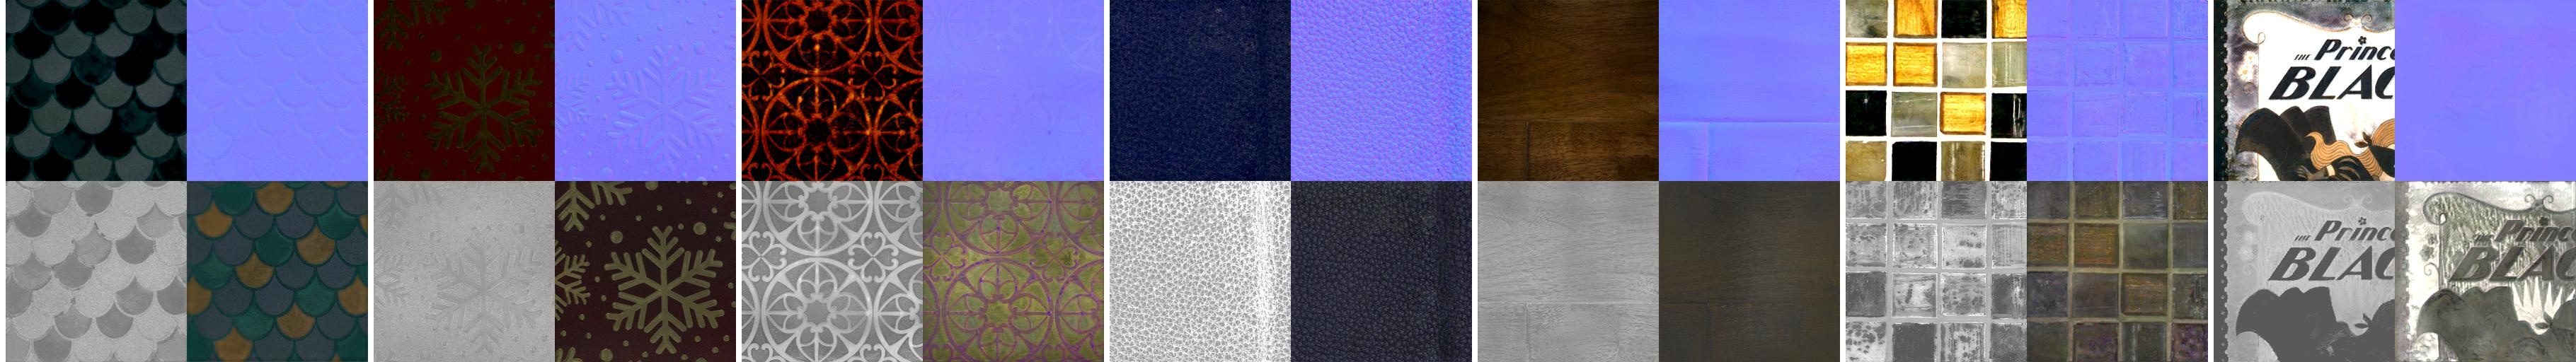
\includegraphics[width=\resLen]{teaser/maps.jpg}
				\end{tabular}
			\end{figure}
	        
	        \vspace{1cm}
    
            \large{
	            We introduce a method to capture SVBRDF material maps from a small number of mobile flash photographs, achieving high quality results both on original and novel views. Our key innovation is optimization in the latent space of MaterialGAN, a generative model trained to produce plausible material maps; MaterialGAN thus serves as a powerful implicit prior for result realism. Here we show re-rendered views for several different materials under environment illumination. We use 7 inputs for these results (with 2 of them shown).
	            (Please use Adobe Acrobat and click the renderings to see them animated.)
            }

        \end{block}
        
        \vspace{1cm}
        
        \begin{block}{MaterialGAN}
            \large{
				A GAN that is trained to generate plausible materials, thus implicitly learning an SVBRDF manifold. 
				MaterialGAN is based on the architecture of StyleGAN2 \cite{karras2020}.
				
				\vspace{1cm}
				
				\textbf{The capability of MaterialGAN generator:}
			}
		
	        \setlength{\resLen}{1.8in}
			\begin{figure}
				\centering
%				\addtolength{\tabcolsep}{-4pt}
				\begin{tabular}{ccccccc}
					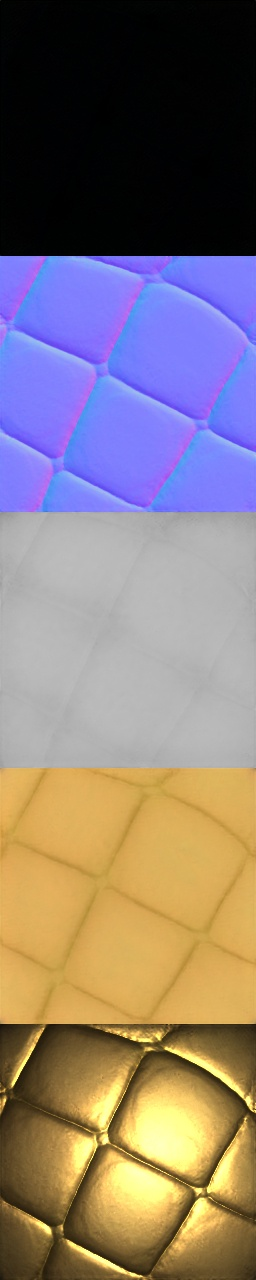
\includegraphics[width=\resLen]{others/matgan/04.jpg} &
					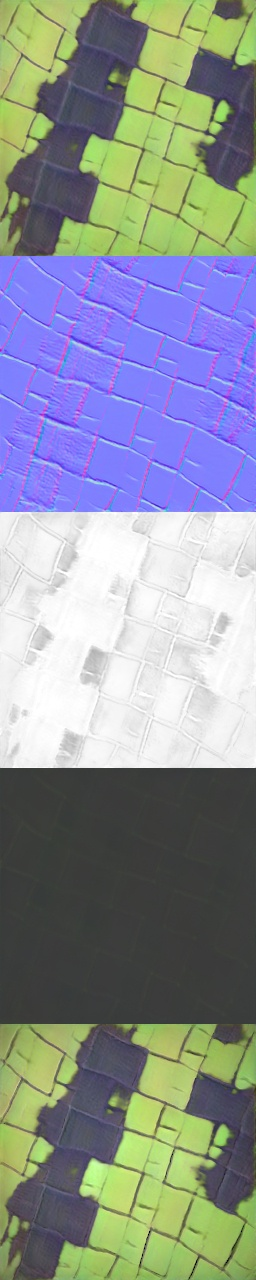
\includegraphics[width=\resLen]{others/matgan/05.jpg} &
					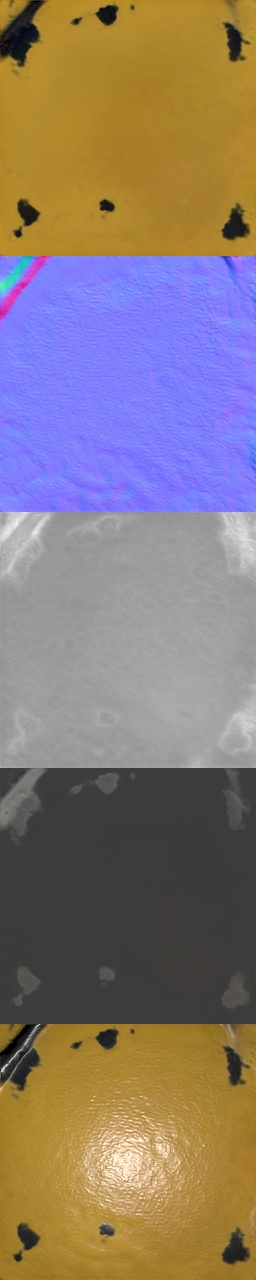
\includegraphics[width=\resLen]{others/matgan/08.jpg} &
					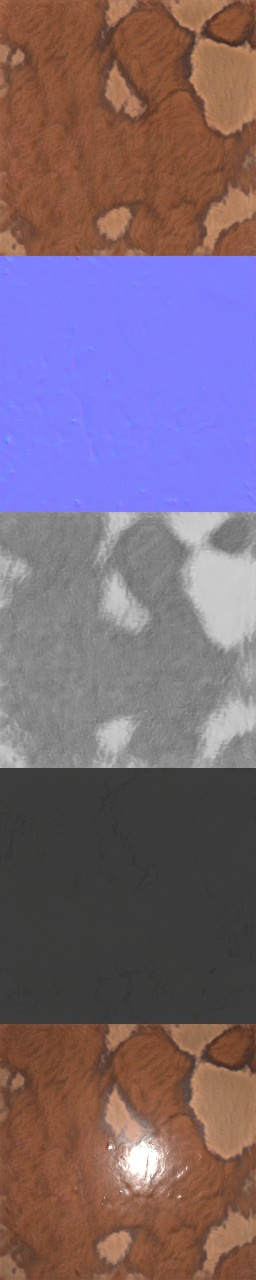
\includegraphics[width=\resLen]{others/matgan/10.jpg} &
					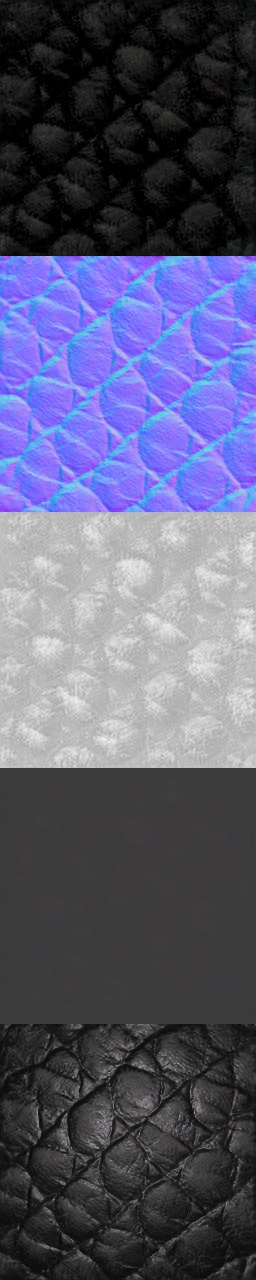
\includegraphics[width=\resLen]{others/matgan/11.jpg} &
					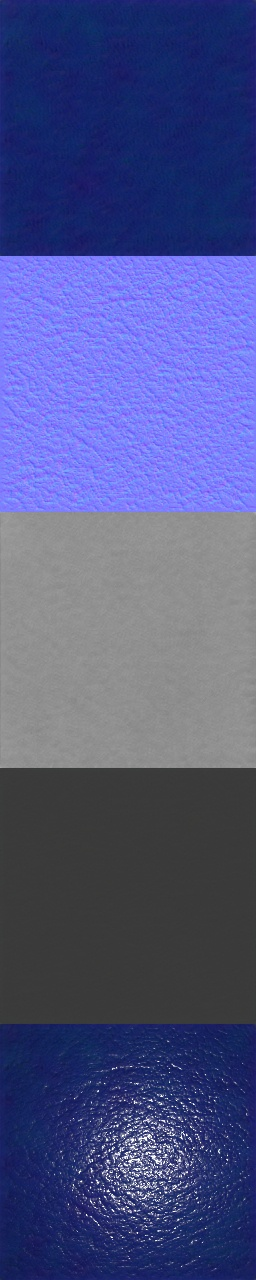
\includegraphics[width=\resLen]{others/matgan/12.jpg} &
					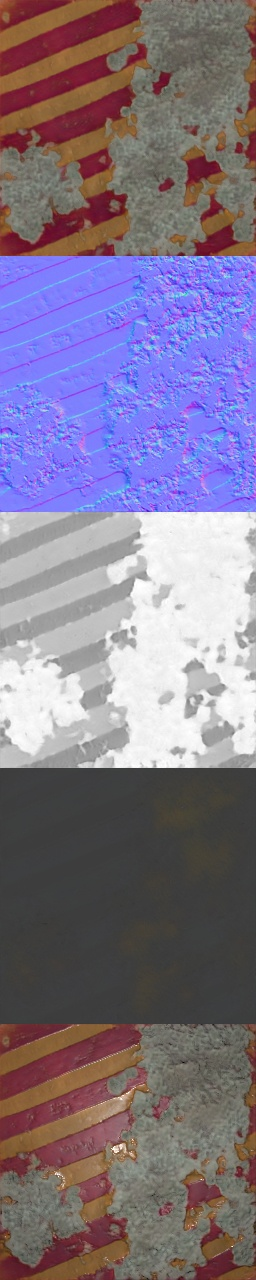
\includegraphics[width=\resLen]{others/matgan/19.jpg}
				\end{tabular}
			\end{figure}
		
			\large{
				The material maps generated by randomly sampling MaterialGAN are high-quality with meaningful correlations both spatially and across materials parameters, and visually look like plausible real-world materials.
			}
		
        \end{block}
    \end{column} % End of the first column
    
    %----------------------------------------------------------------------------
    %        MIDDLE
    %----------------------------------------------------------------------------
    \begin{column}{\sepwid}\end{column} % Empty spacer column
    \begin{column}{\twocolwid} % Begin a column which is two columns wide (column 2)
        \begin{block}{Inverse rendering}
        	\large\textbf{Pipeline:}
        	
			\begin{figure}
				\centering
				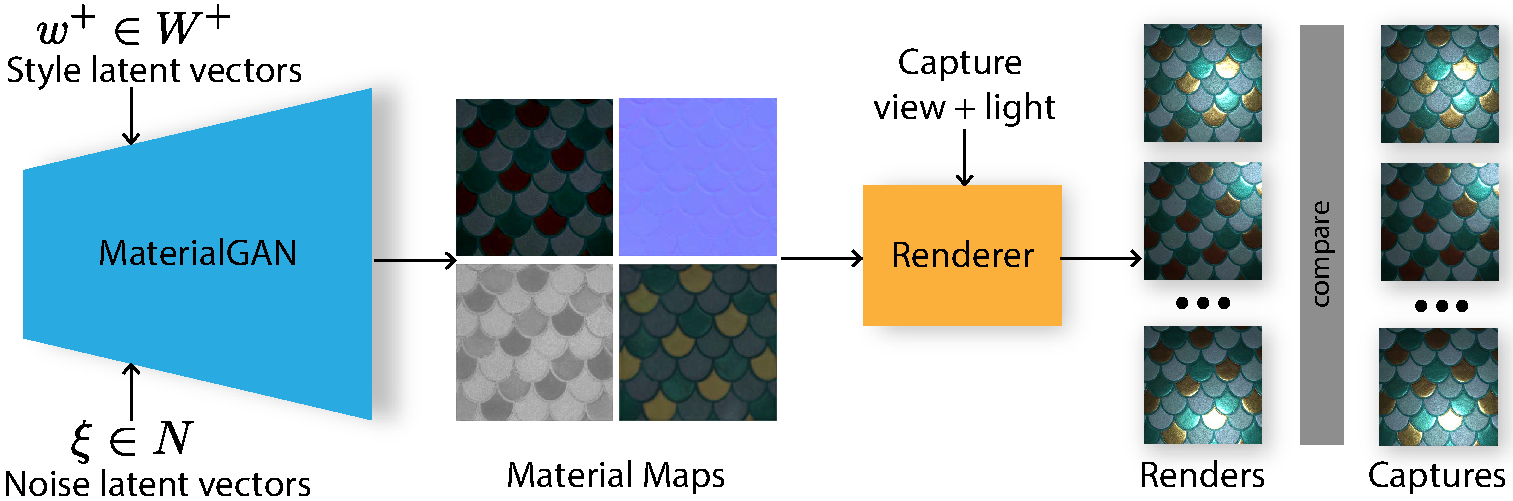
\includegraphics[width=14in]{others/system.pdf}
			\end{figure}
		
			\large{
				We optimize for latent vectors $\bm{w}^+$ and $\bm{\xi}$, 
				that feed into the layers of the StyleGAN2-based MaterialGAN model. 
				The MaterialGAN generator produces material maps (diffuse albedo, normal, roughness and specular albedo),
				that are rendered under the captured view/light settings. 
				Finally, the renderings and measurements are compared using a combination of L2 and perceptual losses.
			}
	
		\end{block}
	
        \vspace{0.5cm}
        
        \begin{block}{Comparison}
            \large\textbf{Ours is less sensitive to initialization:}
            
			\begin{figure}
				\centering
				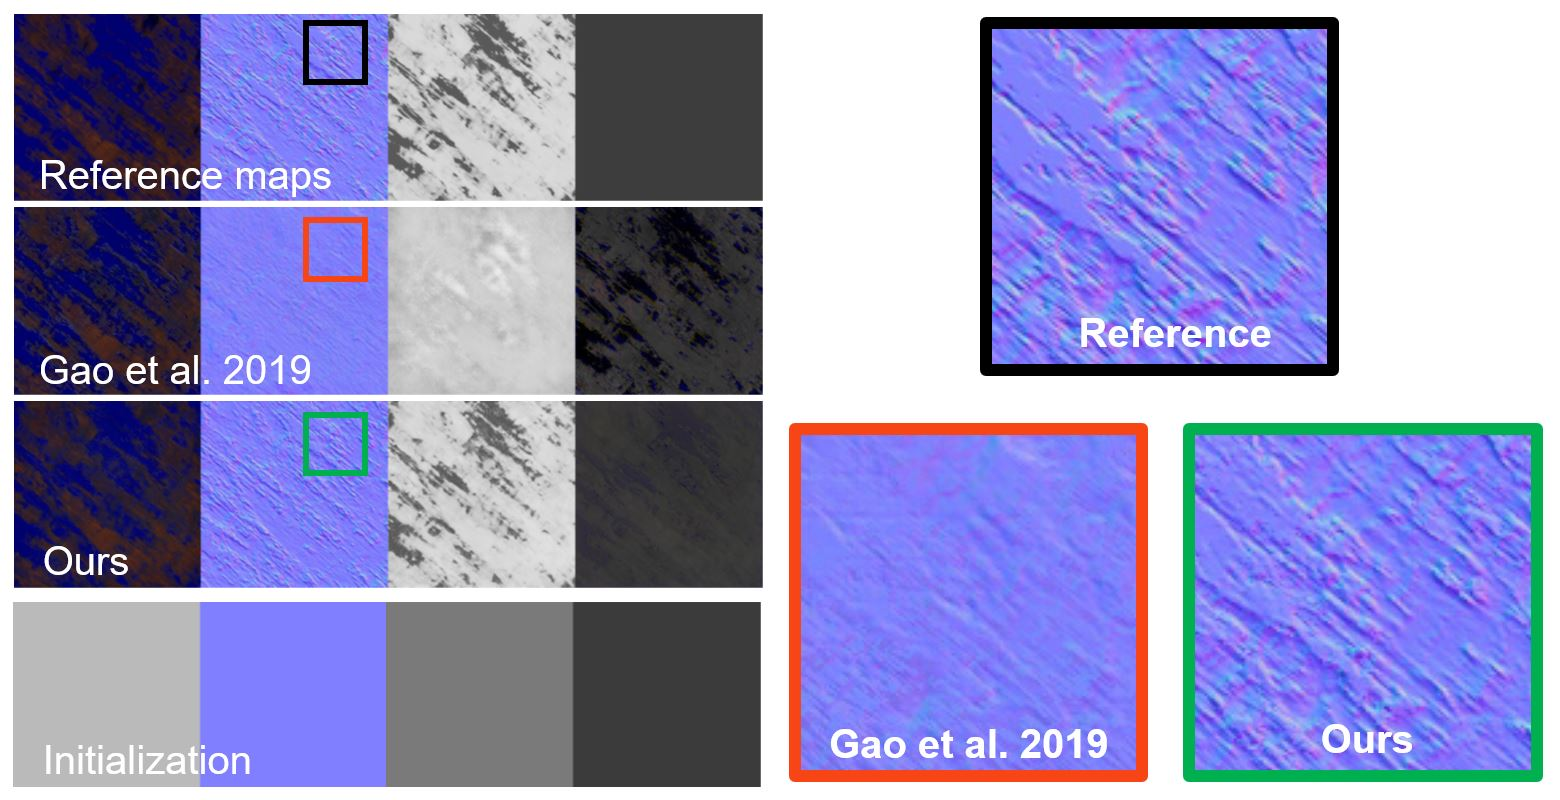
\includegraphics[width=14in]{results/init.jpg}
			\end{figure}
            
            \vspace{1cm}

            \large{\textbf{Post-refinement is less important in ours method:}}

			\begin{figure}
				\centering
				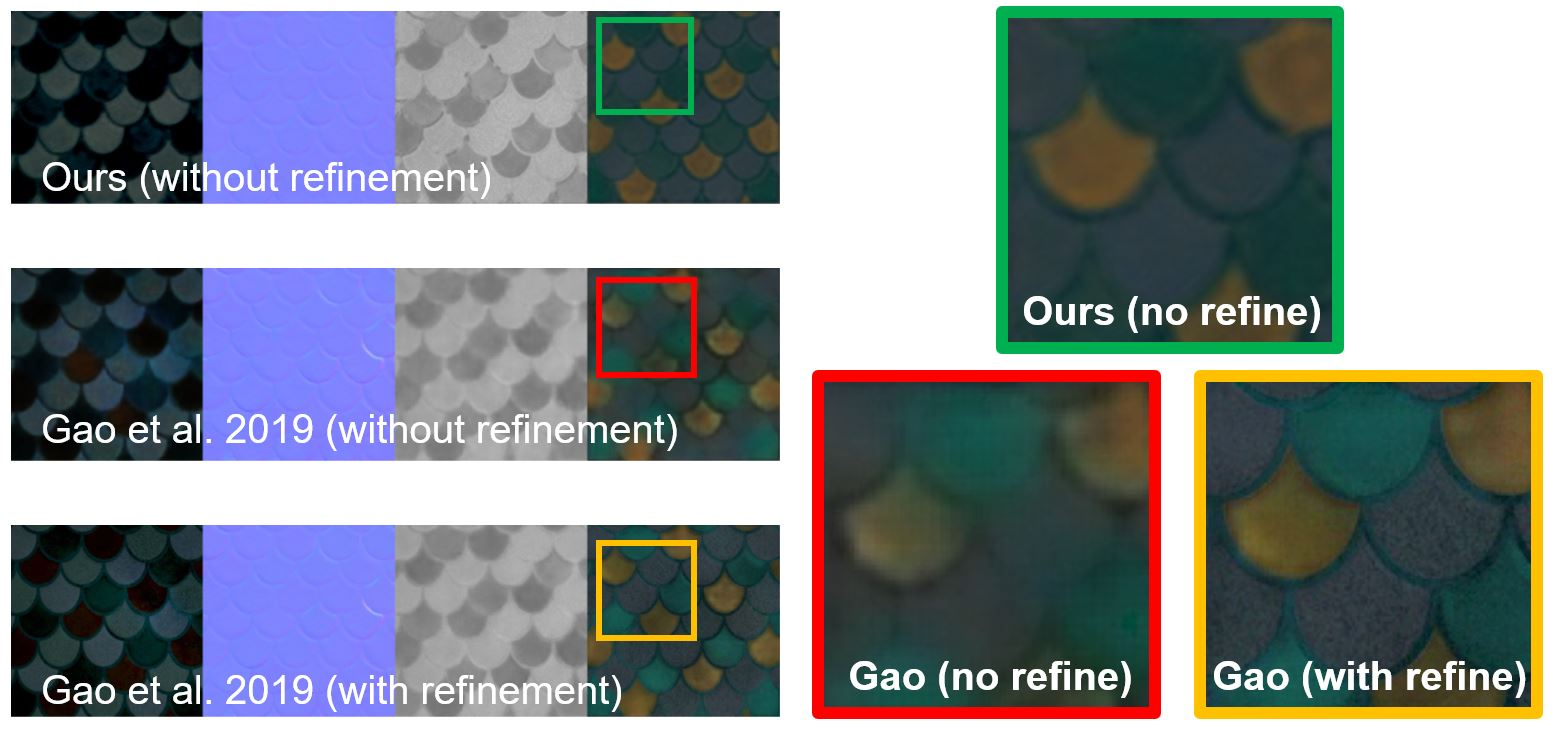
\includegraphics[width=14in]{results/post.jpg}
			\end{figure}

        \end{block}
    \end{column}
    
    %----------------------------------------------------------------------------
    %	RIGHT
    %----------------------------------------------------------------------------
    \begin{column}{\sepwid}\end{column} % Empty spacer column
    \begin{column}{\twocolwid} % The third column
        \begin{block}{Results}
            \large\textbf{Large features:}
            \begin{figure}
				\centering
				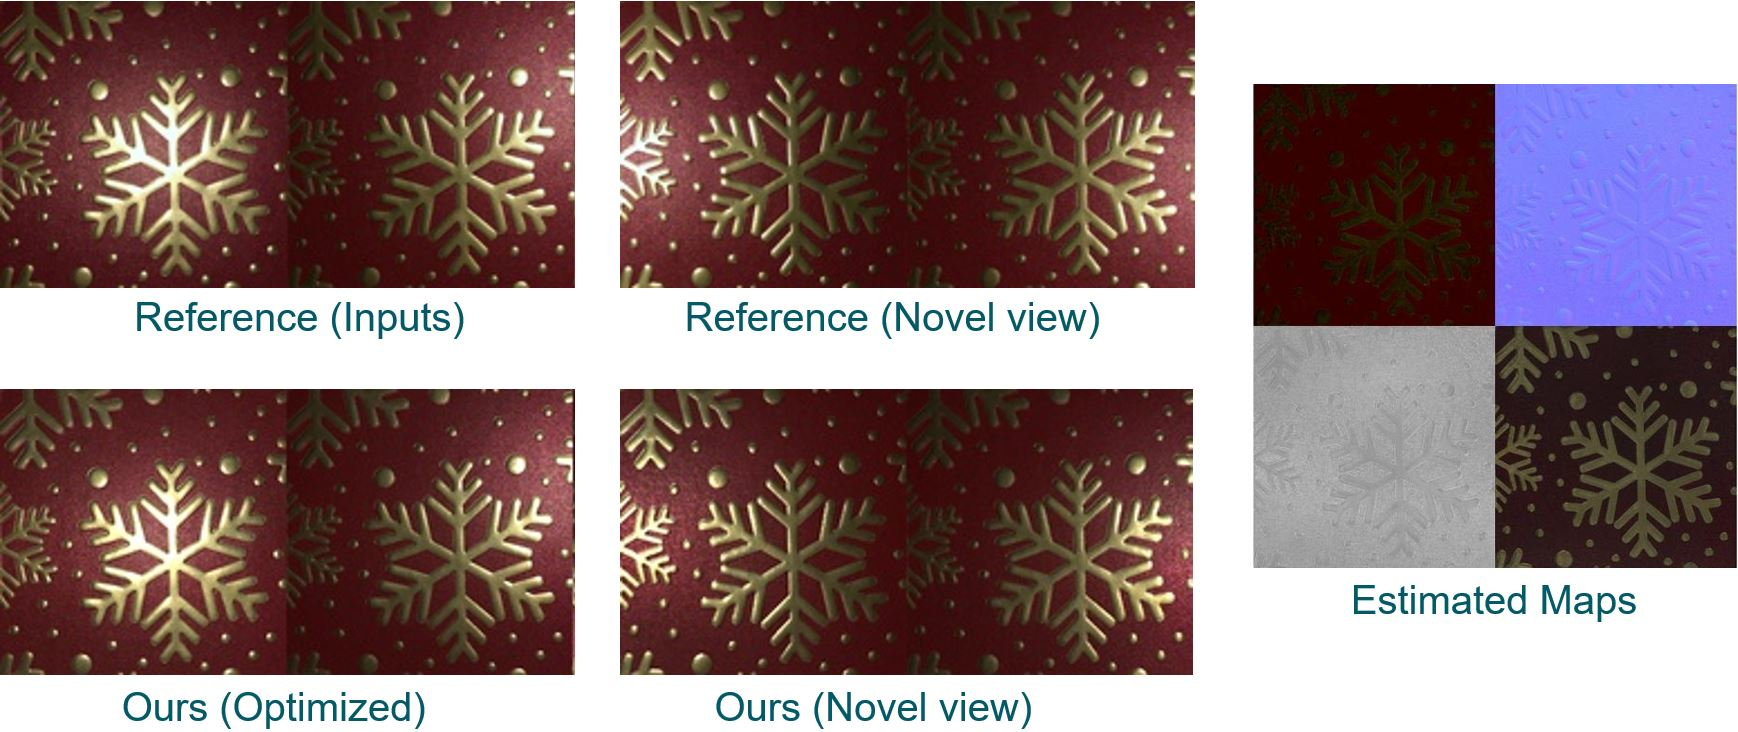
\includegraphics[width=14in]{results/card.jpg}
            \end{figure}
            
%            \vspace{0.5cm}

            \large\textbf{Small features:}
			\begin{figure}
				\centering
				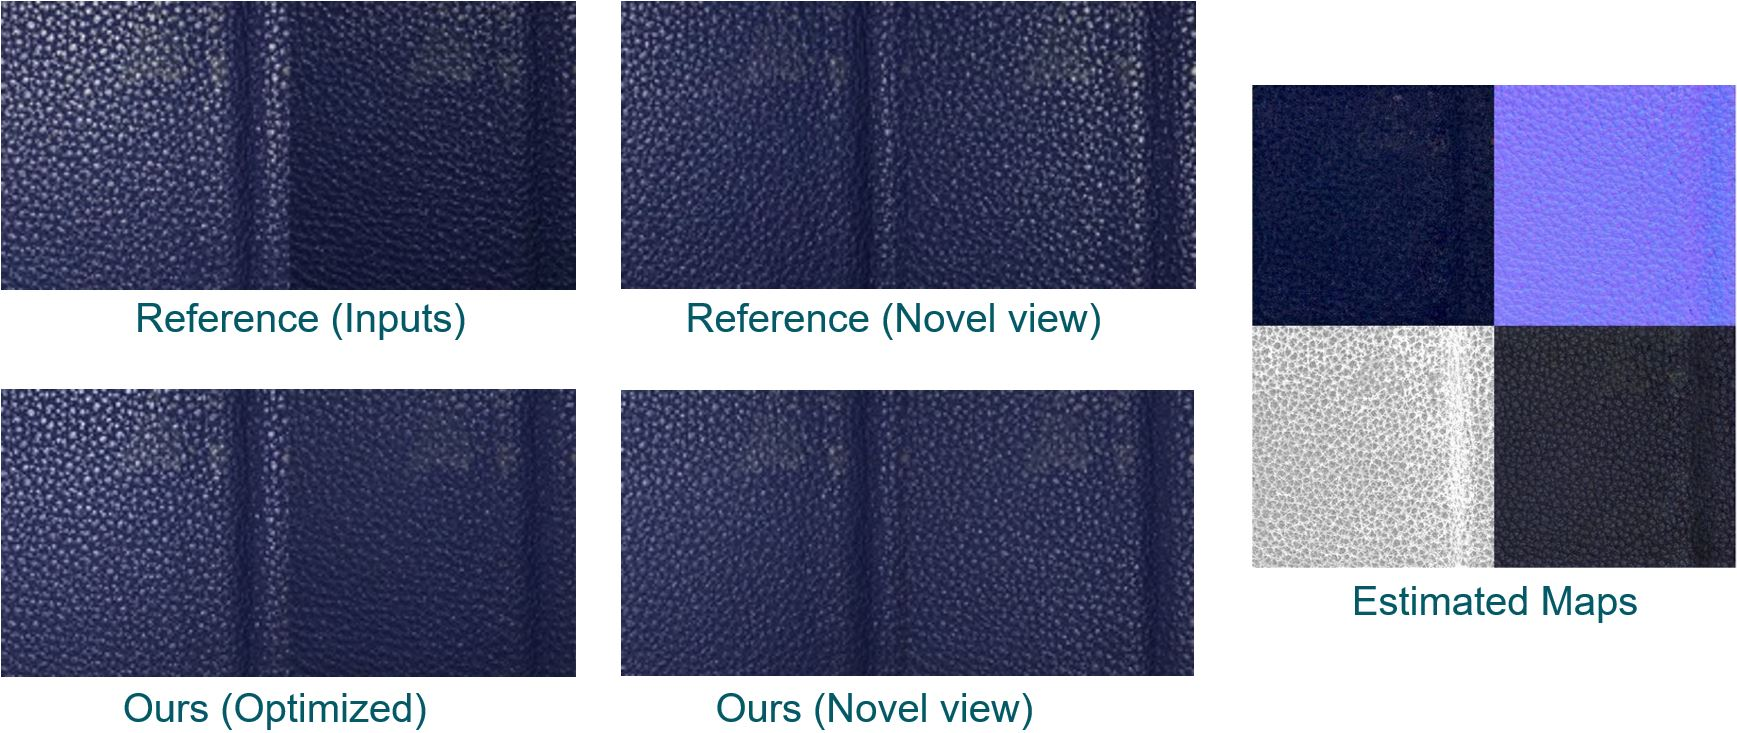
\includegraphics[width=14in]{results/leather.jpg}
			\end{figure}
			
%			\vspace{0.5cm}            

            \large\textbf{High specularity:}
			\begin{figure}
				\centering
				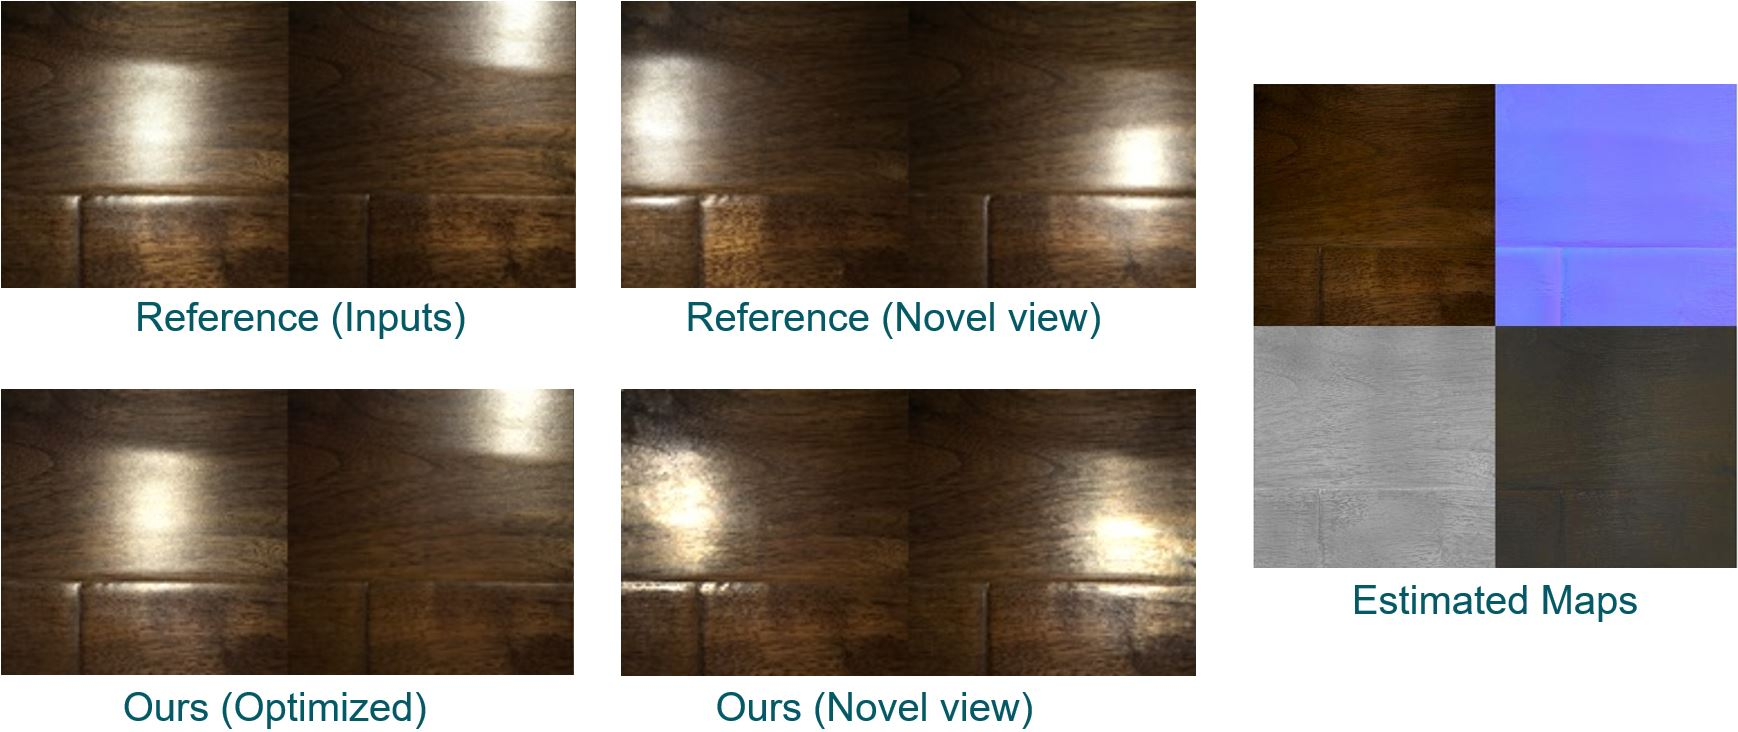
\includegraphics[width=14in]{results/wood.jpg}
			\end{figure}
					
%			\vspace{0.5cm}
			
			\small{(Please see more results from our paper and supplemental materials.)}	
			
        \end{block}

        \begin{block}{References}
            \vspace{-1cm}
            \nocite{*} % Insert publications even if they are not cited in the poster
            \bibliographystyle{unsrt}
            \bibliography{references.bib}
        \end{block}
    \end{column} % End of the third column
    
\end{columns} % End of all the columns in the poster


\end{frame} % End of the enclosing frame
\end{document}